\begin{figure}[h]
\centering
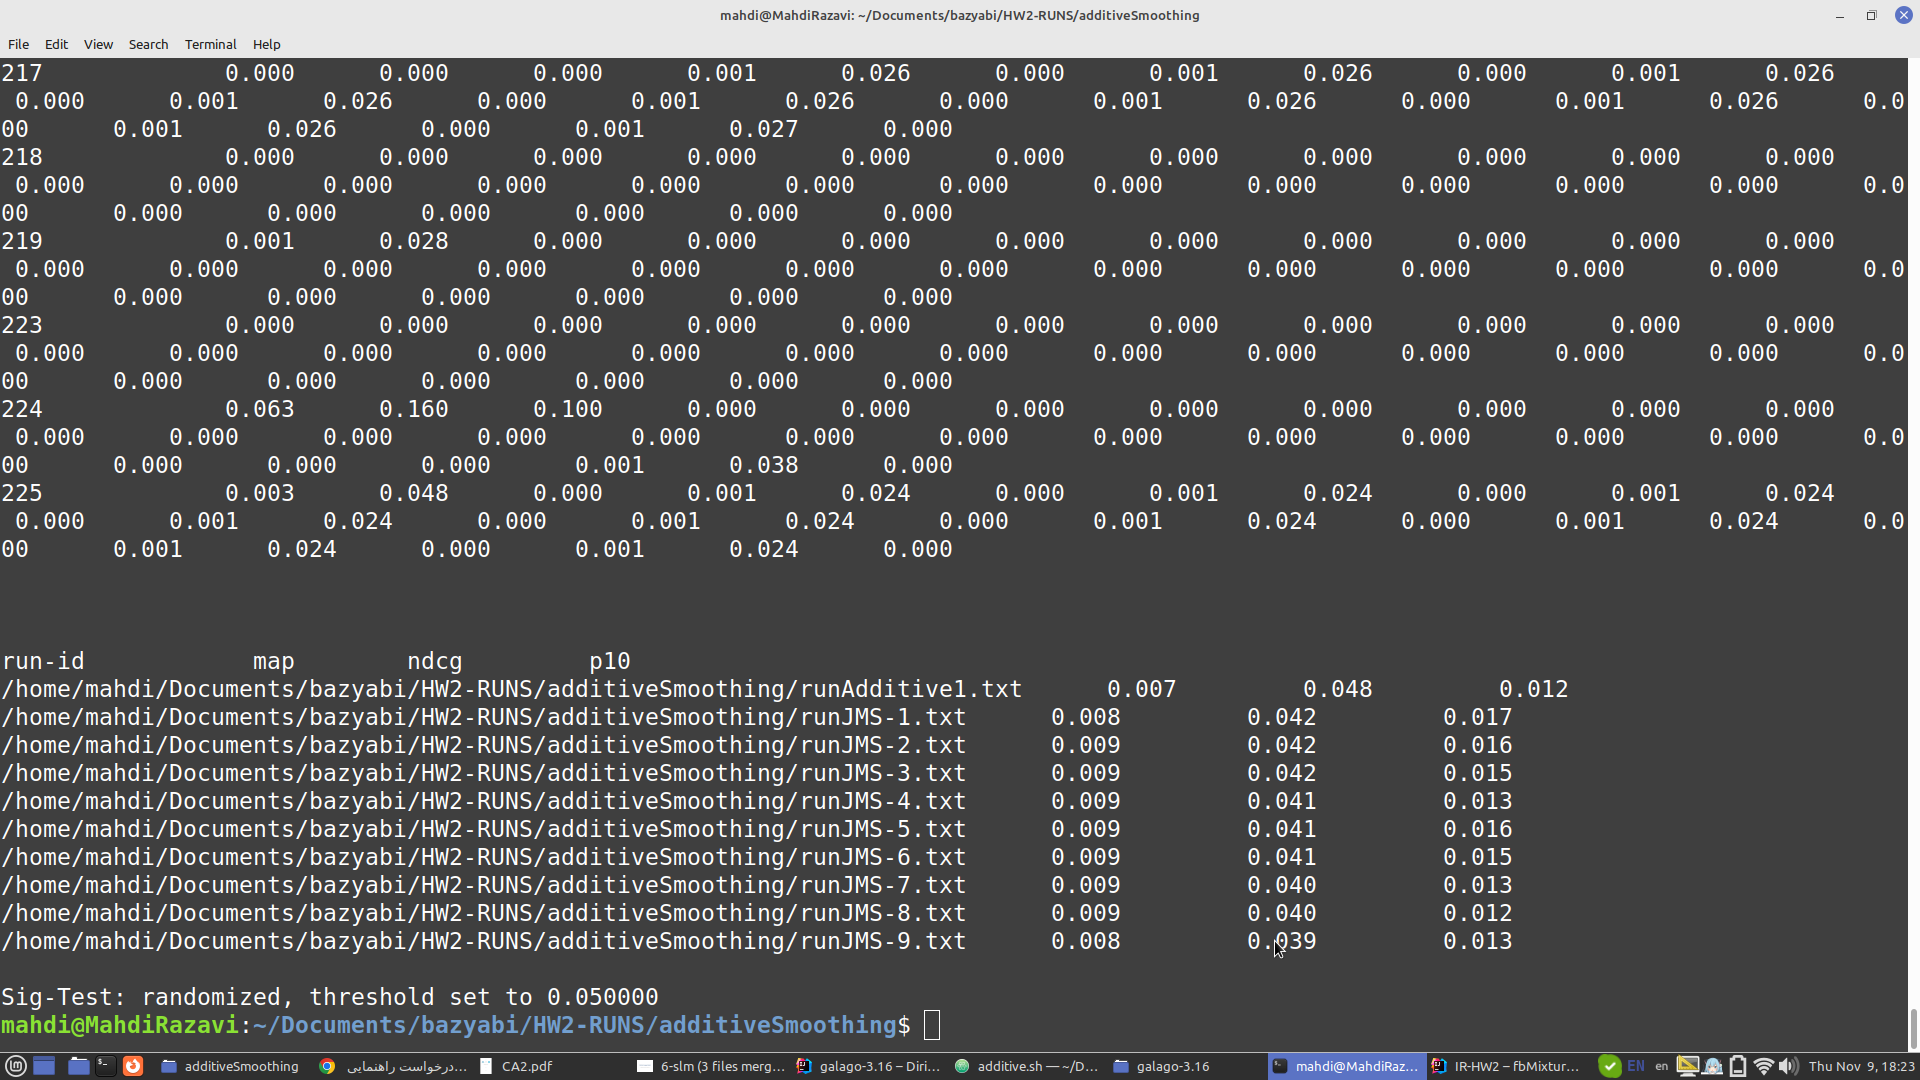
\includegraphics[width=0.8\textwidth]{IR2/images/JMSmothing-Additive0.png}
\caption{
\lr{Additive , JM Smoothing}
}
\end{figure}

\begin{boxM}
    از آنجایی که
    \lr{Additive Smoothing}
    هیچ وابستگی به متغیرهای 
    لاندا و مو
    ندارد ، آن را فقط یکبار آزمایش خواهیم کرد.

    درباره مقایسه روش هموارسازی 
    \lr{Additive}
    در مقایسه با
    \lr{JM Smoothing}
    نمی‌توان کاملا به قطعیت نظرداد چون دچار اختلاف بین پارامترها هستیم.

    برای سهولت امر تست پارامترهای مختلف ، اسکریپت آن را نوشته‌ام.
    پارامترهای متناظر مو و لاندا را با توجه به بازه‌های آن‌ها بررسی خواهیم کرد.

    همانطور که از پارامترها مشاهده می‌شود ، در 
    \lr{JM Smoothing}
    تغییر محسوسی در میزان دقت و سایر پارامترهای متناظر ایجاد نشده است ، اما با نگاهی ریزبینانه تر متوجه خواهیم شد که
    با
    \color{purple}
         افزایش میزان متغیر لاندا 
    ، میزان دقت تابع امتیازدهی به اسناد رو به
    کاهش 
    می‌باشد.

\end{boxM}

\begin{figure}[h]
    \centering
    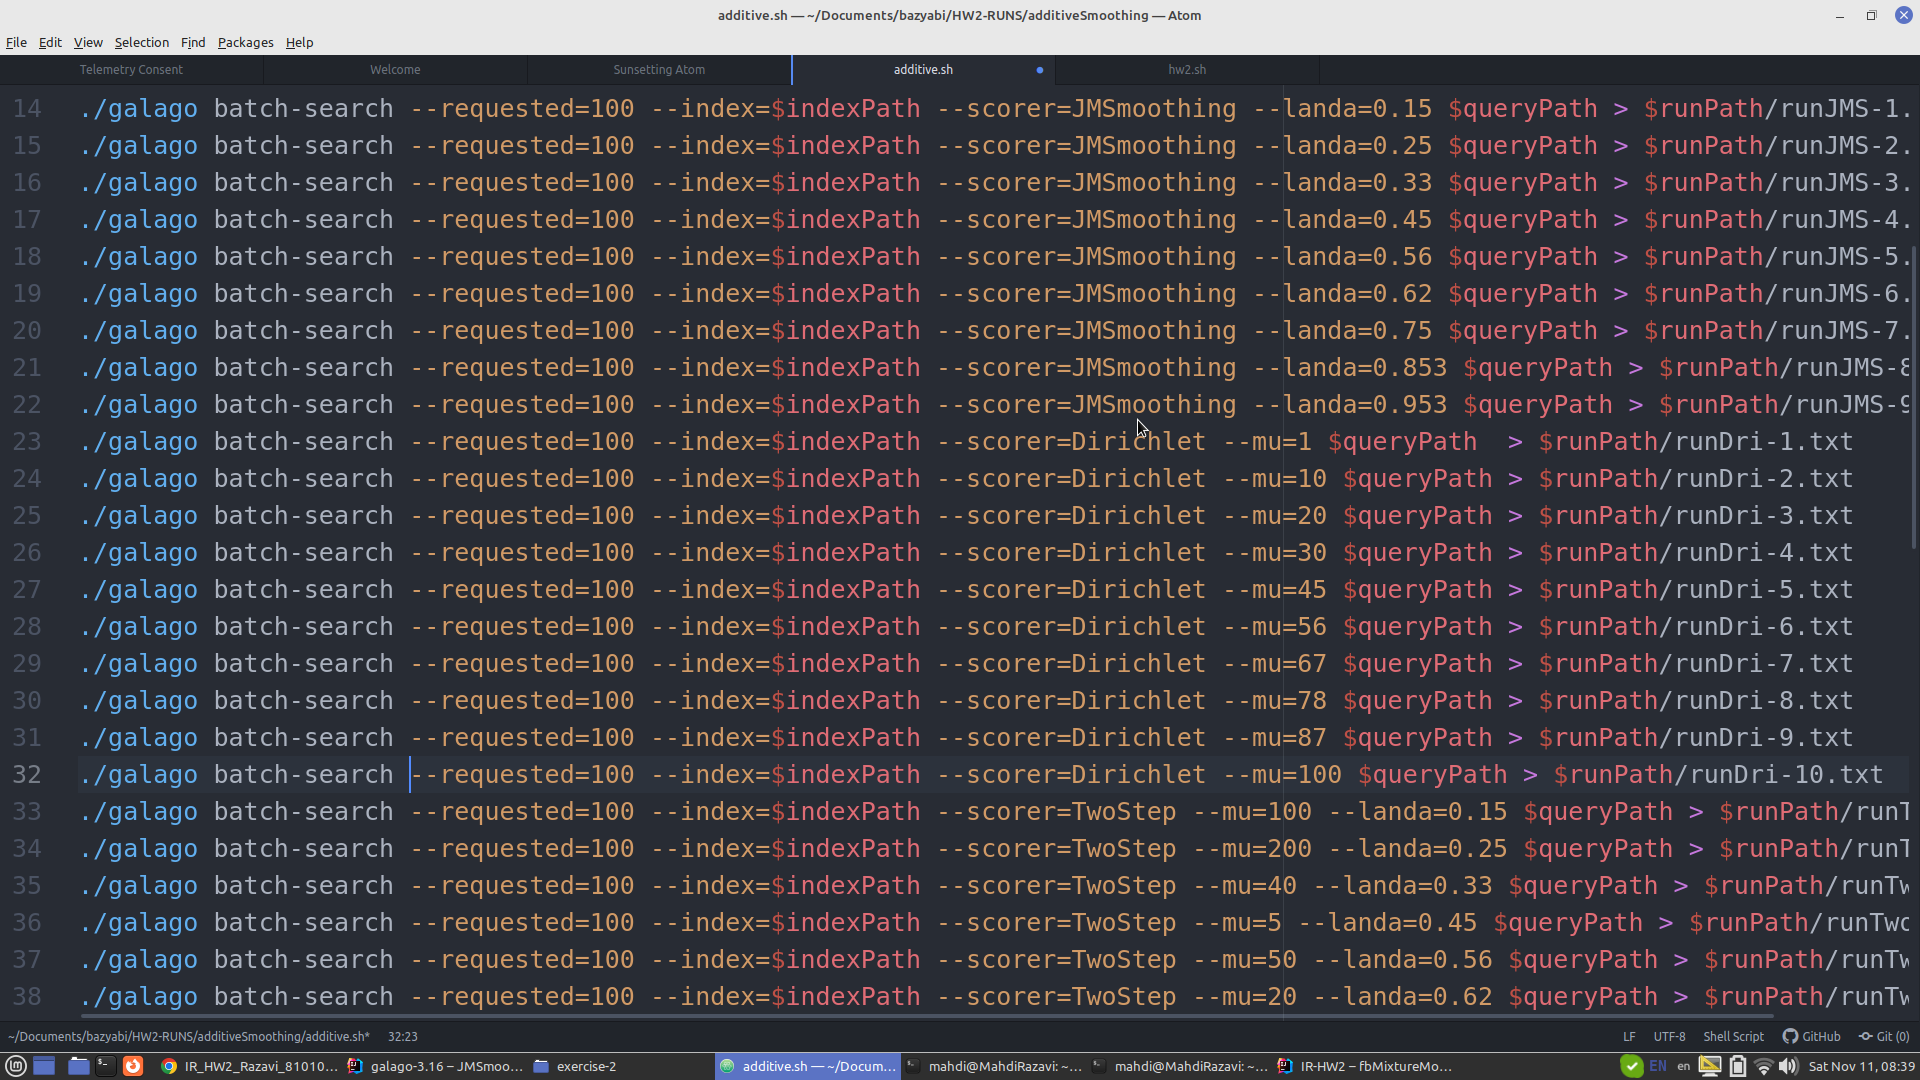
\includegraphics[width=0.8\textwidth]
    {IR2/images/bash-script.png}
    \caption{اسکریپتی برای آزمایش روش‌های هموارسازی}
    \label{fig:enter-label}
\end{figure}

\newpage

\begin{figure}[h]
    \centering
    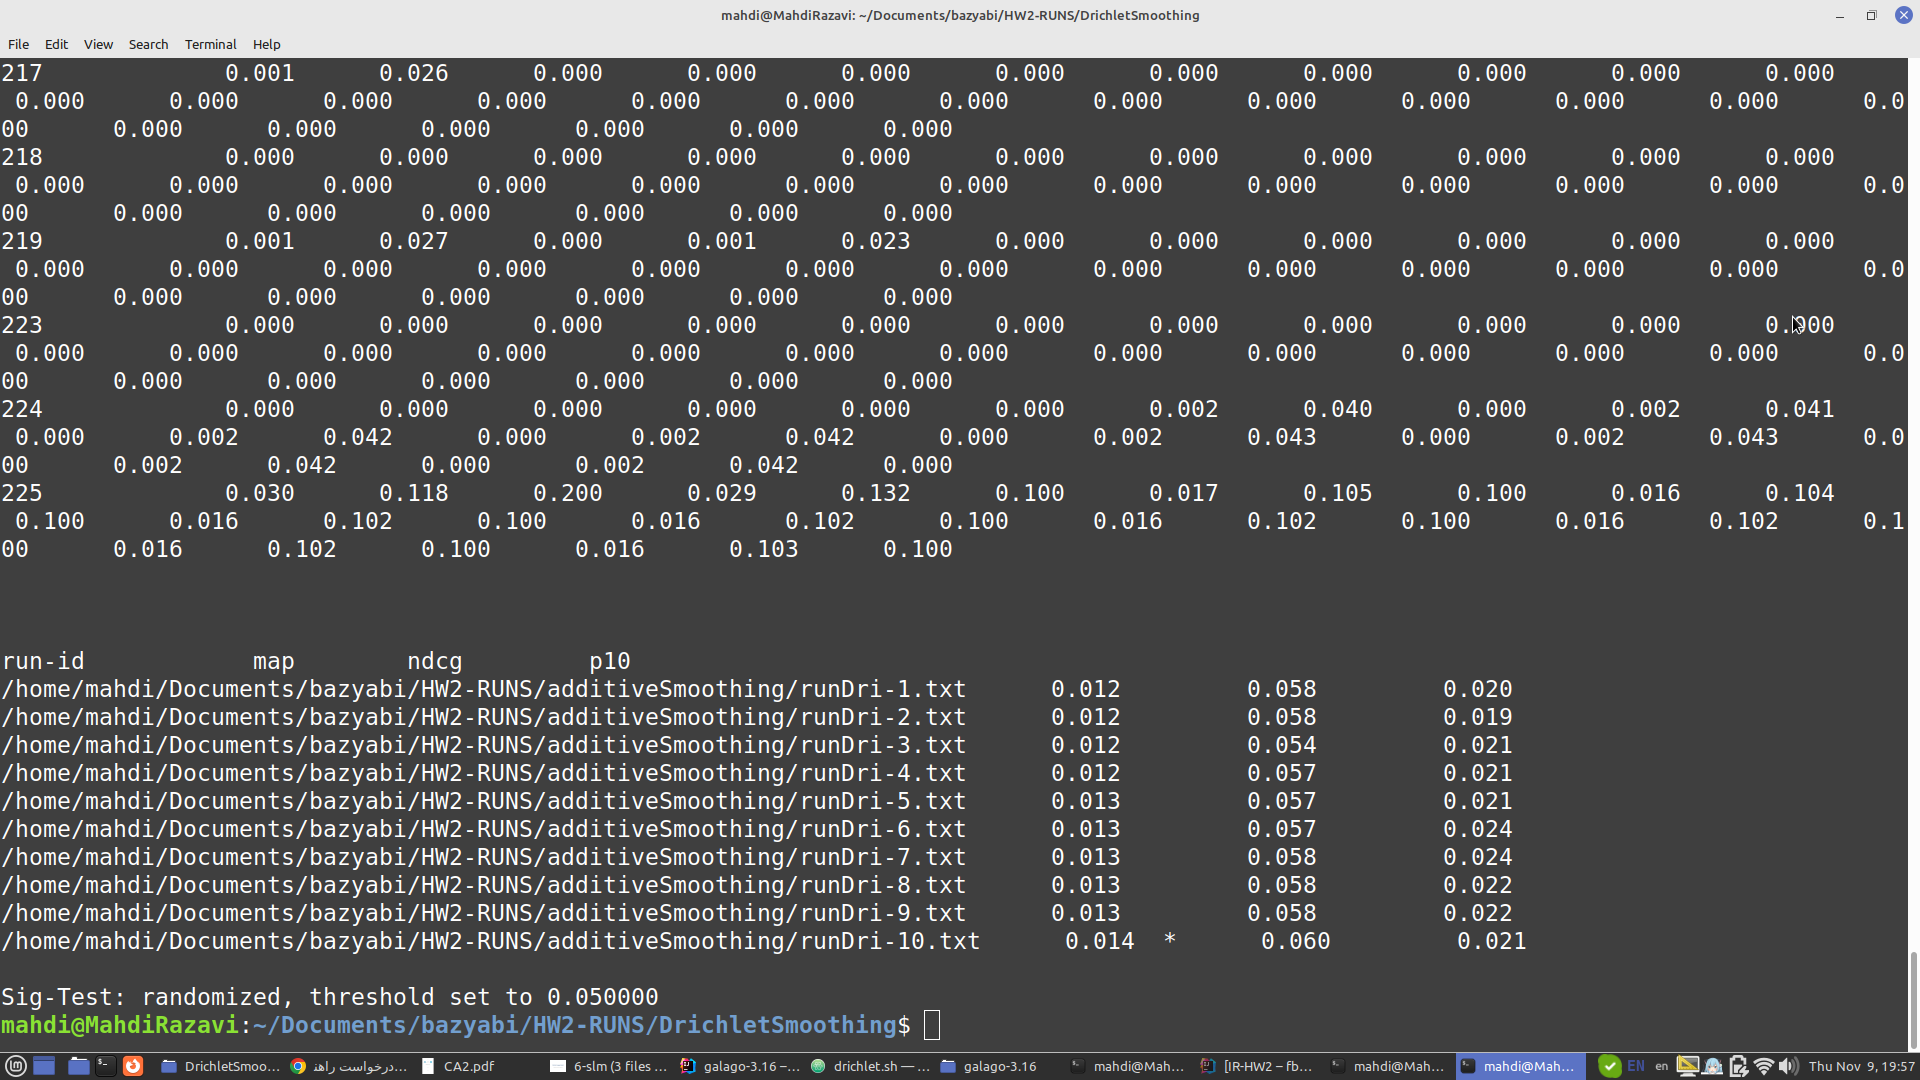
\includegraphics[width=0.8\textwidth]
    {IR2/images/Drichlet.png}
    \caption{\lr{Drichlet Smoothing}}
    \label{fig:enter-label}
\end{figure}

\begin{boxM}
    در این روش هموارسازی ، همانطور که مشخص است بهترین اجرای ما مربوط به اجرای 6 می باشد.
    با توجه به این که مقدار متغیر 
    مو
    در اینجا برابر 56 می باشد و ما در این سری آزمایش ها کلا بازه انتخابی برای 
    متغیر
    مو
    را بین 1 تا 100 در نظرگرفته ایم ، 
    مو
    اینطور به نظر می رسد که در حالت وسط نتیجه متغیرهای مربوط به دقت بازیابی بهتر خواهد بود.
\end{boxM}

\newpage

\begin{figure}[h]
    \centering
    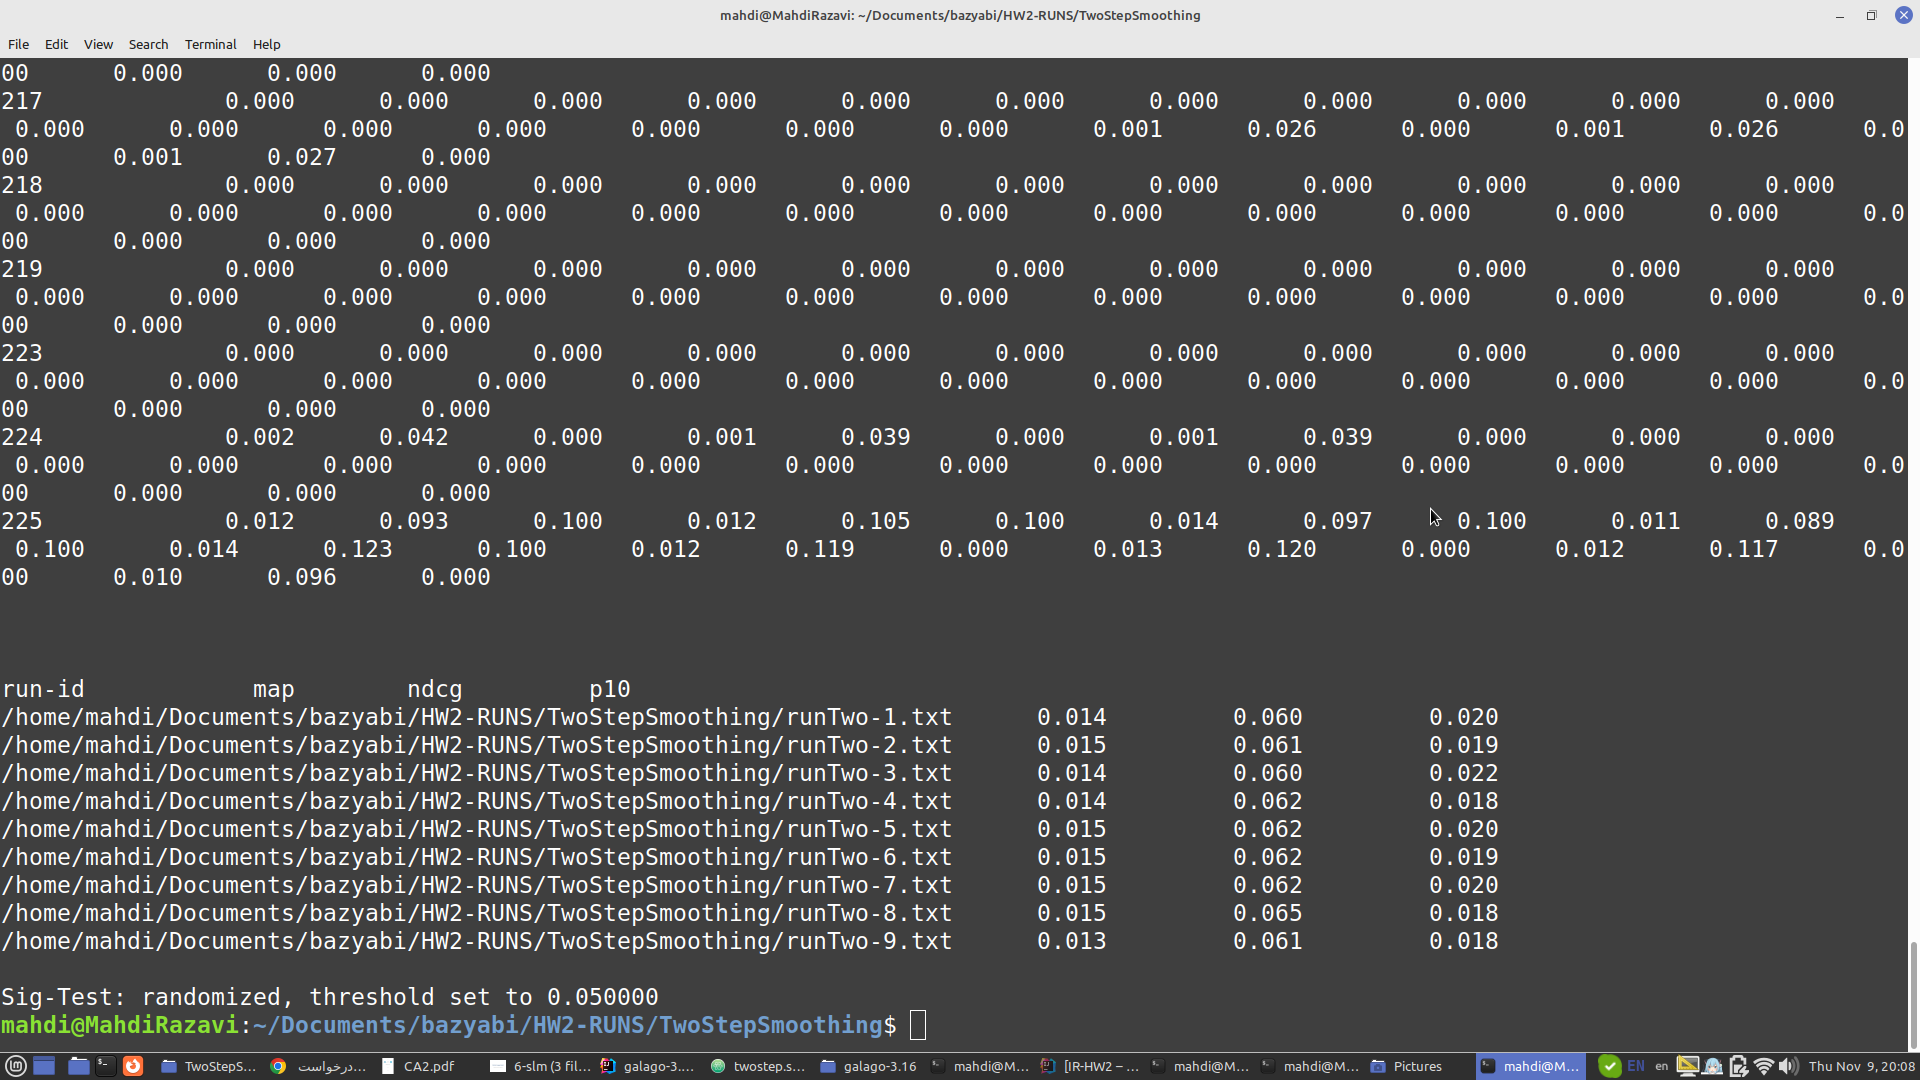
\includegraphics[width=0.8\textwidth]{IR2/images/twoStep.png}
    \caption{\lr{TwoStep Smoothing}}
    \label{fig:enter-label}
\end{figure}

\begin{boxM}
  با توجه به تصاویر بالا بهترین حالت اجرا مربوط به اجرای هشتم می شود.
  متغیر
  لاندا برابر 
  \lr{0.853} 
  و متغیر مو برابر 30 می باشد.

  این نتایج با توجه به حالت های مختلف به دست آمده است.
\end{boxM}

\newpage